\section{Background Research \& Analysis}

\subsection{Application Research \& Analysis}
This section details the research behind the data used in OptiCaff, including the data source, calendar data and the caffeine calculations that will be used in the prototype. 

\subsubsection{Data Source}
\label{sec:Data}
OptiCaff uses the Open Data Service from the University of Southampton \cite{DataSouthampton} to retrieve the relevant information for the application. This service provides open linked data about some of the administrative information regarding the university. It also provides a SPARQL Endpoint \cite{SotonSparql} (a service which facilitates users querying a knowledge base using the SPARQL query language) \cite{SparqlEndpoint}. OptiCaff utilises this with a few specialist queries, and combined with user preferences can provide the user with a wide selection of caffeine choices around campus. 

\subsubsection{Calendar Research \& Analysis}
\label{sec:calendar}
OptiCaff’s initial objectives included the use of university timetables to schedule caffeine level notifications. 
`SUSSED' is the University of Southampton's student portal that displays a student’s timetable. 
Using this web portal is currently the only way to obtain a student's timetable given that it's not freely available as open data or through an API. 
Another University of Southampton produced application, iSoton, has been able to do this process showing that it is possible.
Further investigation however has shown that this is not a trivial process. 

Instead an alternative solution is to use Android Calendar which synchronises to maky calendar systems \cite{calendar}.
Overall given the prototype nature of this application and ability to use Google Calendar in a much simpler fashion it was decided that OptiCaff would use Android Calendar. 

\subsubsection{Caffeine Research \& Analysis} 
\label{sec:Caffeine}
In order to provide the caffeine management element of this application, the different levels of caffeine that appear in beverages and its effect on human beings needed to be researched.
This section details the caffeine levels and decay rate that have been used in OptiCaff. 

Given the vast range of different caffeinated products and the limited time to produce a prototype application, it was decided that the products displayed by OptiCaff would be grouped into four different types of drink, and each type would be allocated an average caffeine content. Below is a table showing these totals, which were obtained these sources \cite{Coke} \cite{TeaCoffee} \cite{EnergyDrink}.

\begin{center}
\begin{tabular}{|l|l|}
\hline
\textbf{Drink Category} & \textbf{Average Caffeine Content (mg)} \\\hline
Tea & 40 \\\hline
Coffee & 54 \\\hline
Energy Drinks & 80 \\\hline
Soft Drinks & 34.5 \\\hline
\end{tabular}
\end{center}

In addition to calculating the level of caffeine obtained from a specific product, it was also important to work out the optimum caffeine levels and how long it would take the caffeine to ``decay" within the body so that the next caffeine consumption time could be predicted. 
For the purposes of the prototype, OptiCaff uses optimum caffeine levels of between 100mg and 200mg. 
The half life of caffeine ranges between 2.5 and 4.5 hours \cite{CaffeinePharmacology} \cite{CaffeinePharmacy}. 
4 hours was chosen as the number to use in OptiCaff and was calculated using the half life formula detailed in \cite{HalfLife}.
 
\subsection{Market Research \& Analysis}
This section details the market research analysed for OptiCaff.
The Coffee market was researched as were the mobile development platforms. 
Finally the potential competitors to OptiCaff are detailed and analysed to see if any of them offer a similar user experience. 

\subsubsection{Coffee Research \& Analysis}
Coffee consumption in the United Kingdom has steadily increased over the past decade. 
In particular the past five years have seen an explosive increase, there are several theories as to why this is the case.
Firstly, instant coffee shops have become more common on our high streets. 
Companies such as Starbucks and Costa have been opening more stores as more citizens have been buying instant coffee; this doesn’t show any signs of slowing down either as Starbucks have recently announced 300 new stores to be opened over the next five years \cite{starbucks}.

Secondly, these brands have contributed to the newfound ‘coolness’ that is associated with coffee \cite{popular}. 
Lastly, there is evidence that the economic climate has played a part in coffee’s rise. 
Also known as the ‘lipstick effect’, Britons have been unable to afford expensive treats for themselves so they have been spending on cheaper treats, a good example of which is coffee \cite{costa}.
This research is important to OptiCaff because it shows that the coffee industry is on the rise, and it would not make business sense for us to invest in a declining industry.

\subsubsection{Mobile Platform Research}
\label{sec:Mobile}
OptiCaff’s purpose heavily lent itself to being a mobile application. 
There are various mobile operating systems that OptiCaff could be deployed on \cite{differentOS}: Google's Android, Apple's iOS, Blackberry's RIM and Windows Mobile. 

The Smartphone Operating System statistics from June 2011 showed Android and Apple dominating the market at present (shown in figure \ref{fig:Mobile}).
Therefore these two platforms were considered.

\begin{figure}[ht]
\begin{center}
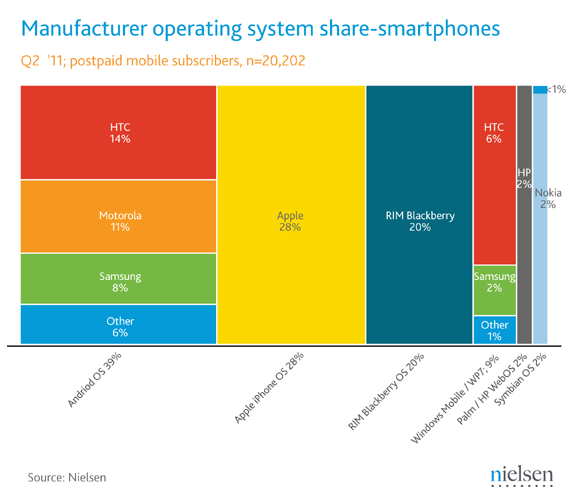
\includegraphics[trim = 0mm 20mm 0mm 30mm, clip, scale=0.5]{images/smartphone.png}
\caption{Manufacture Operating System Share Smartphones June 2011 \cite{smartphone}}
\label{fig:Mobile}
\end{center}
\end{figure}

The following elements were considered in regards to which platform to use: language, development requirements and popularity of the apps for that operating system.

\textbf{Programming Language}
\begin{itemize}
	\item{iOS for iPhone requires applications to be written in Objective C \cite{objectivec}.}
	\item{The Android Operating System requires applications to be written in Java \cite{AndroidSDK}.}
\end{itemize}

\textbf{Development Requirements}
\begin{itemize}
	\item{The only IDE available for developing iPhone applications is XCode which relies on having Apple's iOS SDK installed \cite{iOS}. Both of these are only available to Apple Mac Computers.}
	\item{Android doesn't require any special hardware to develop an application. The Android SDK is freely available and its recommended development enviroment Eclipse \cite{Eclipse} is also free.}
\end{itemize}

\textbf{Application Popularity}
\begin{itemize}
	\item{Apple's App Store is currently the more popular at 25 billion downloads \cite{AppleDownload}}
	\item{Google Play (Android's market place) was reported to have reached 10 billion downloads in December 2011 \cite{AndroidDownload}.}
\end{itemize}

It was decided that for the prototype application, Android would be the simpler option for the following reasons:
\begin{itemize}
	\item{Android uses Java. All members of the team are experienced in Java development and one member has experience in Android Development.}
	\item{Android can be developed on any platform which is useful as the group uses a combination of Mac, Linux and Windows.}
	\item{Google Play may be less popular than Apple's app store, however it still holds a large user base and it was decided that ease of development was a higher priority for the prototype.}
\end{itemize}

\subsubsection{Gamification Research \& Analysis}
A common issue for new apps is user retention; a method of increasing this is Gamification \cite{gamification1}. Gamification is the practise of adding game-like elements to something that is not already a game, e.g. a to-do list \cite{gamification2}. There are ways in which gamification can be applied to OptiCaff.

\begin{enumerate}
	\item{Use of achievements or awards. Achievements are used to recognise when a player has fulfilled certain conditions when playing a game (e.g OptiCaff could award achievements to the users that remain in the optimum caffeine range for 3 hours).}
	\item{Use of leaderboards. A leaderboard would show the users that are the best at using OptiCaff in a specified way, (e.g. showing users who stay in the optimum range for the longest time.}
\end{enumerate}

Based on this research, it was decided that OptiCaff would use leaderboards as a method of gamification, provided that it is done safely. 
This is because leaderboards can link all of OptiCaff's users turning it into a multiplayer game. 
Obviously, as with any game there would be the potential to cheat by pressing the button without actually consuming the caffeine, but this still doesn't detract from the fun element. 
One of the dangers of gamification is extreme behaviour, OptiCaff will not reward behaviour that is potentially dangerous, e.g. rewarding the user that has the highest caffeine intake.

\subsubsection{Monetisation Research \& Analysis}
It is more challenging to profit from Android Applications compared to Apple iOS Applications according to a report from Distimo, an app store analysis company \cite{monetisiation}. 
The report suggests several methods to maximise the money earned.

\begin{enumerate}
	\item{80\% of paid applications have been bought less than 100 times.}
	\item{The profits of in-app advertising vary greatly, depending on user base size.}
	\item{It is common in app stores/marketplaces to have a paid version of an app alongside a free version. There is no difference in the functionality of the app, though the paid version does not display advertisements.}
\end{enumerate}

Based upon these three points it has been decided that OptiCaff would be developed as a free and paid version, containing advertising in the free version.
The next logical step after gaining a significant user base would be to pitch the application to caffeine vendors for funding in exchange for favouring their points of service within the application.  

\subsubsection{Competitors Research \& Analysis}
\label{sec:competitors}
This section details both the direct and indirect competitors to Opticaff and ascertains if any of them offer a similar user experience. 

Caffeine Finder is a BlackBerry application, and is a direct competitor of OptiCaff. 
Caffeine Finder directs a user to the nearest restaurant or café, give the address and even display reviews of the destination if available. 
There are however several negative points regarding this application:
\begin{itemize}
	\item{BlackBerry has a small screen compared to Android phones and iPhones.} 
	\item{The application doesn’t inform the user of the optimum time to consume caffeine.}
	\item{A user may already be tired before they think to check Caffeine Finder which is something OptiCaff will try and prevent.} 
	\item{The application was released in 2005 and has not been updated regularly since that time, this is shown by reports that it is not fully compatible with newer operating systems.}
\end{itemize}

Caffeine Zone 2 Lite is a free iPhone application that tracks the amount of caffeine in the body, OptiCaff will also have caffeine tracking.. 
Making Caffeine Zone 2 Lite a direct competitor, although OptiCaff offers a superior service for the following reasons:  
\begin{itemize}
	\item{OptiCaff offers a complete solution, Caffeine Zone 2 Lite only tells the user when they should have caffeine, it doesn't tell the user where they can get a caffeinated drink.} 
	\item{The alerts generated do not consider the user’s schedule, OptiCaff will look at the user’s calendar to see if they require an earlier warning for caffeine to accomodate their schedule.}
	\item{Caffeine Zone 2 Lite is focused on being an educational tool for caffeine use. This is in contrast to OptiCaff which will prioritise providing a service.}
\end{itemize}

One of the issues of using open data is that the data itself can be considered an indirect competitor of OptiCaff. It could be possible for another product to be created using the same data set, this means that OptiCaff could have more potential competitors than it would if it used closed data. 
 
Table \ref{tab:Competitors} summarises the competative edge of Opticaff, illustrating how it combines the key features of its competitors into a superior all encompassing service:

\begin{table}[ht]
\caption{Table of Opticaff's Competitors}
\label{tab:Competitors}
\begin{tabular}{|p{240pt}| p{40pt} | p{40pt} | p{40pt} | p{40pt} |}
    \hline
     	& 
	Caffeine Finder & 
	Caffeine Zone & 
	Caffeine Data & 
	Opticaff
\\ \hline
   	Does this app allow you to locate caffeine sources? & 
	\LARGE{\textcolor{green}{\Pisymbol {pzd} {52}}} & 
	\LARGE{\textcolor{red}{\Pisymbol {pzd} {56}}} &
	\LARGE{\textcolor{green}{\Pisymbol {pzd} {52}}} & 
	\LARGE{\textcolor{green}{\Pisymbol {pzd} {52}}}
\\ \hline
    Does this app help you to manage caffeine content? & 
	\LARGE{\textcolor{red}{\Pisymbol {pzd} {56}}} & 
	\LARGE{\textcolor{green}{\Pisymbol {pzd} {52}}} & 
	\LARGE{\textcolor{red}{\Pisymbol {pzd} {56}}} &
 	\LARGE{\textcolor{green}{\Pisymbol {pzd} {52}}}
\\ \hline
    	Does this app help you to manage caffeine content in relation to your day's activities? & 
	\LARGE{\textcolor{red}{\Pisymbol {pzd} {56}}} & 
	\LARGE{\textcolor{red}{\Pisymbol {pzd} {56}}} &
	\LARGE{\textcolor{red}{\Pisymbol {pzd} {56}}} &
 	\LARGE{\textcolor{green}{\Pisymbol {pzd} {52}}}
\\ \hline
\end{tabular}
\end{table}
